\documentclass[simple]{eskdtext}



%\usepackage{amsmath,amsthm,amssymb} % formulas
%\usepackage{unicode-math}
%\usepackage{mathtools}
\usepackage{tinos}
%\usepackage{fontspec}
%\setmainfont{Times New Roman}
%\setsansfont{Verdana}
%\setmonofont{Courier New}
%\newfontfamily{\cyrillicfonttt}{tinos}
%\usepackage{polyglossia} % for russian hyphenation
%\setmainlanguage{russian}
%\setotherlanguage{english}

\usepackage{xecyr}
\usepackage{xunicode,xltxtra}


% packages
%
% Тестовое наполнение текстом
% При написании работы - удалить пакет и комманды \lipsum
\usepackage{lipsum}
%
\usepackage{graphicx}
\usepackage{datetime}
\usepackage{enumitem} % for lists
\usepackage{ulem} % for underlining
\usepackage{lastpage} % Number of pages
\usepackage{hyperref} % Links in pdf

% fix eskdx
\makeatletter
\newsavebox\ESKDpicturebox
\renewcommand{\ESKD@ShipoutPicture}{%
     \ifESKD@twoside
       \ifodd\c@page
         \ESKDframeX=\ESKD@margin@si
       \else
         \ESKDframeX=\ESKD@margin@so
       \fi
     \else
       \ESKDframeX=\ESKD@margin@si
     \fi
     \ESKDframeY=\ESKD@margin@b
     \ESKDstampX=\ESKDframeX
     \advance\ESKDstampX \ESKDframeW
     \advance\ESKDstampX -185mm
     \ESKDstampY=\ESKDframeY    
     \sbox\ESKDpicturebox{%
        \unitlength=1mm
        \begin{picture}(0,0)(\ESKDltu{\ESKD@origin@x},\ESKDltu{\ESKD@origin@y})%
          \ifx\ESKD@thisstyle\@empty
            \let\ESKD@thisstyle\ESKD@curstyle
          \fi
          \loop
          \ifnum \ESKD@hash@pos{@style@draw@\ESKD@thisstyle} %
            < \ESKD@hash@count{@style@draw@\ESKD@thisstyle}
            \ESKD@hash@next@value{@style@draw@\ESKD@thisstyle}\relax
          \repeat
          \ifx\ESKD@extra@ThisHook\@empty%
            \ESKD@extra@Hook\else\ESKD@extra@ThisHook%
          \fi%
          \global\let\ESKD@thisstyle\@empty%
          \global\let\ESKD@extra@ThisHook\@empty%
        \end{picture}
        }%
       \AddToHook{shipout/foreground}{%
       \put(1in,-1in){\usebox\ESKDpicturebox}}%        
}
\makeatother



% setup
\newcommand{\FrontPageDepartment}{ИТ} %Факультет
\newcommand{\FrontPageSubdepartment}{ИС} %Кафедра
\newcommand{\WorkType}{Курсовой проект} %Тип работы (заголовок)
\newcommand{\Subject}{Предмет} %по ... родительный падеж
\newcommand{\Topic}{Тема курсового проекта} %Тема
\newcommand{\Professor}{Иванов~И.~И.} %Руководитель
\newcommand{\Student}{Петров~П.~П.} %Студент
\newcommand{\Group}{ИСм-112} %Группа
\ESKDsignature{МИВУ 230400.68 ПЗ} % Код специальности и тип работы
\newcommand{\FrontPageDate}{\ddmmyyyydate\today} %Дата

% eskdx setup
\ESKDletter{}{У}{}
\ESKDtitle{\WorkType\\\Topic}
\ESKDchecker{\Professor}
\ESKDauthor{\Student}
\ESKDcolumnIX{МИ ВлГУ\\ \Group}

\addto\captionsrussian{\def\refname{Список использованных источников}}
\sloppy % split long lines

% graphics path
\graphicspath{{src/img/}}


% verbatim setup
\newcommand{\verbatimFont}{
\fontsize{10pt}{12pt}\selectfont
\baselineskip=1em
}


% workaround for regression in babel package on linux
\providecommand{\No}{\textnumero}


% remove vertical space from lists
\renewcommand{\alph}[1]{\asbuk{#1}} % костыль для кирилической нумерации вместо латинской
\setlist{nolistsep} % убираем дополнительные вертикальные отступы вокруг списков
\setenumerate[1]{label=\alph*), fullwidth, itemindent=\parindent,  listparindent=\parindent}
\setenumerate[2]{label=\arabic*), fullwidth, itemindent=\parindent, listparindent=\parindent, leftmargin=\parindent}
\setitemize{fullwidth, itemindent=\parindent, listparindent=\parindent}

\lstdefinestyle{cpp}{
  belowcaptionskip=1\baselineskip,
  breaklines=true,
  frame=L,
  numbers=left,
  xleftmargin=\parindent,
  language=C++,
  showstringspaces=false,
  basicstyle=\scriptsize,
  keywordstyle=\bfseries\color{green!40!black},
  commentstyle=\itshape\color{purple!40!black},
  identifierstyle=\color{blue},
  stringstyle=\color{orange},
}


% main document
\begin{document}
% Титул
\ESKDthisStyle{title}
\newlength{\frontpagefk} % Ширина поля Факультет/Кафедра
\setlength{\frontpagefk}{6cm}
\newlength{\frontpagerb} % Ширина надписей Руководитель/Студент и пр. под темой
\setlength{\frontpagerb}{6cm}
\newlength{\frontpagerbspace} % ??? (do not remove)
\setlength{\frontpagerbspace}{1cm}
\newlength{\FrontPageSubjSpace} % Ширина пробела до и после названия предмета
\setlength{\FrontPageSubjSpace}{1cm}
\newlength{\FrontPageTopicSpace} % Ширина пробела до и после темы
\setlength{\FrontPageTopicSpace}{0.5cm}

\thispagestyle{empty}
\begin{center}
{
\vspace*{-1.5cm}
\baselineskip=1.3em
{\small Министерство образования и науки Российской Федерации}\\
\textbf{Муромский институт (филиал)}\\
{\footnotesize федерального государственного бюджетного образовательного учреждения\\
высшего образования}\\
\textbf{<<Владимирский государственный университет\\
имени Александра Григорьевича и Николая Григорьевича\\
Столетовых>>\\
(МИ ВлГУ)\\}
}

\bigskip
\begin{tabular}{l c}
\textbf{Факультет}&\underline{\makebox[\frontpagefk]{\FrontPageDepartment}}\\
\textbf{Кафедра}&\underline{\makebox[\frontpagefk]{\FrontPageSubdepartment}}\\
\end{tabular}

\vspace{\fill}
\begin{Huge}
\textsl{\WorkType}
\end{Huge}

\vspace{\fill}
по \underline{\makebox[\FrontPageSubjSpace]{}\Subject\makebox[\FrontPageSubjSpace]{}}

\smallskip
\parbox{15cm}{\centering{Тема: \uline{\makebox[\FrontPageTopicSpace]{}\Topic\makebox[\FrontPageTopicSpace]{}}}}

\vspace{\fill}

\begin{flushright}
\makebox[\frontpagerb][c]{
\makebox[\frontpagerb][l]{Руководитель}\hspace{\frontpagerbspace}}

\smallskip
\makebox[\frontpagerb][c]{
\raisebox{-\baselineskip}{\shortstack{\underline{\makebox[\frontpagerb][l]{\Professor}}\\
\begin{footnotesize}
(фамилия, инициалы)
\end{footnotesize}}}\hspace{\frontpagerbspace}}

\bigskip
\makebox[\frontpagerb][c]{
\raisebox{-\baselineskip}{\shortstack{\underline{\makebox[\frontpagerb][l]{}}\\
\begin{footnotesize}
(подпись)\hfill(дата)
\end{footnotesize}}}\hspace{\frontpagerbspace}}

\newcommand{\frontpagerbstudent}[2]{ %
\makebox[\frontpagerb]{ %
\raisebox{-\baselineskip}{\shortstack{#1\ \underline{\makebox[\frontpagerb-\widthof{#1\ }][c]{#2}}\\
\begin{footnotesize}
\makebox[\widthof{#1\ }][c]{}\makebox[\frontpagerb-\widthof{#1\ }][c]{(группа)}
\end{footnotesize}}}\hspace{\frontpagerbspace}}
}

\bigskip
\makebox[\frontpagerb][c]{\frontpagerbstudent{Студент}{\Group}}

\smallskip
\makebox[\frontpagerb][c]{
\raisebox{-\baselineskip}{\shortstack{\underline{\makebox[\frontpagerb][l]{\Student}}\\
\begin{footnotesize}
(фамилия, инициалы)
\end{footnotesize}}}\hspace{\frontpagerbspace}}

\renewcommand{\dateseparator}{.}

\bigskip
\makebox[\frontpagerb][c]{
\raisebox{-\baselineskip}{\shortstack{\underline{\makebox[\frontpagerb][r]{\FrontPageDate}}\\
\begin{footnotesize}
(подпись)\hfill(дата)
\end{footnotesize}}}\hspace{\frontpagerbspace}}

\end{flushright}

\vspace{\fill}
Муром -- \the\year
\vspace*{-1cm}
\end{center}
\newpage

% Аннотация
\ESKDthisStyle{empty}
\input{src/annotation.tex}
\newpage

% Содержание
\setcounter{page}{4}
\ESKDthisStyle{formII}
\tableofcontents
\newpage

% Основной текст
\begin{center}
\WorkType

\Topic
\end{center}

мама мыла раму
мама мыла раму
мама мыла раму
мама мыла раму

                   мама                      мыла раму
мама мыла раму
										мама мыла раму
мама 					мыла раму
мама мыла раму



\begin{lstlisting}[style=customc,caption={Листинг программы}]
int main()
{
    printf("Hello, World!");
    return 0;
}
\end{lstlisting}


\begin{figure}[h]
\centering
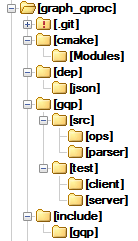
\includegraphics[scale=1]{structure}
\caption{Дерево файлов проекта}
\label{fig:structure2}
\end{figure}


\newpage

% Список литературы
\begin{thebibliography}{00}

\bibitem{bib_name1} источник 1

\bibitem{bib_name2} источник 2

\bibitem{bib_name3} источник 3

\bibitem{wiki_main} Википедия: свободная энциклопедия: на русском языке [Электронный ресурс] // URL:  http://ru.wikipedia.org/wiki/Заглавная\_страница  (дата обращения: 06.05.2013)

%\bibitem{wiki_main} Википедия: свободная энциклопедия: на русском языке [Электронный ресурс] // URL:  http://ru.wikipedia.org/wiki/Заглавная\_страница  (дата обращения: \ddmmyyyydate\today)

\end{thebibliography}

\end{document}